% !TEX program = pdflatex
% !TEX root = staged_reward_paper.tex

\documentclass{article}

% Allow compiling either from paper/ or from the repository root.
\makeatletter
\def\input@path{{./}{paper/}}
\makeatother

\usepackage[preprint,nonatbib]{neurips_2026}

\usepackage[utf8]{inputenc}
\usepackage[T1]{fontenc}
\usepackage[UTF8]{ctex}
\usepackage{amsmath}
\usepackage{amssymb}
\usepackage{booktabs}
\usepackage{graphicx}
\usepackage{tabularx}
\usepackage{array}
\usepackage{makecell}
\usepackage{enumitem}
\usepackage{xcolor}
\usepackage{hyperref}
\usepackage{url}

\graphicspath{{../output/extra_results/poster/}{output/extra_results/poster/}}
\setlist[itemize]{leftmargin=1.5em}
\setlist[enumerate]{leftmargin=1.8em}
\newcommand{\relu}[1]{\left[#1\right]_+}
\newcommand{\ind}{\mathbf{1}}

\title{上半身扰动下人形机器人摆臂行走策略的稳定性}

\author{%
  技术报告 \\
  HumanoidVerse / Genesis / PPO \\
  \texttt{Stable Arm-Swing Humanoid Locomotion under Upper-Body Perturbations}
}

\begin{document}

\maketitle

\begin{abstract}
人形机器人在解锁上半身自由度后，行走控制不再是单纯的下肢速度跟踪问题。上肢动作会改变躯干姿态、角动量分布和足端接触节奏；若直接在基础 locomotion reward 上叠加摆臂目标，策略容易出现侧向漂移、躯干代偿、上肢抖动或摆臂信号被稳定项抑制等问题。本文面向 H1 人形机器人构建了一个三阶段强化学习奖励课程：首先在完整 19DoF 动作空间中约束上半身，学习稳定前向行走；随后借鉴 gait-conditioned reward routing 思想，根据速度命令构造站立、行走和直线行走掩码，仅在适当步态上下文中激活上肢摆臂奖励；最后在动作层对 torso、shoulder 和 elbow 注入随机脉冲扰动，使策略学习扰动后的稳定恢复。实验表明，最终策略在 32 个并行环境、20 s 评估窗口和扰动幅度 2.0 下保持 100\% 存活率，前向速度误差为 0.0245 m/s，最大姿态倾斜低于 10 deg，同时保留可见肩部摆幅和手臂末端前后位移。该结果说明，稳定摆臂行走更适合被建模为一个逐步增强的 reward routing 与鲁棒性学习问题，而不是单一摆臂奖励的权重调节问题。
\end{abstract}

\textbf{关键词：} 人形机器人；强化学习；奖励设计；摆臂；步态条件化；上肢扰动；鲁棒行走

\section{引言}

人形机器人行走策略通常首先追求速度跟踪、姿态稳定和接触可靠性。然而，当任务从下肢行走扩展到全身协调行走时，上半身自由度会显著增加控制问题的复杂度。以 H1 机器人为例，下肢基线只控制 10 个腿部关节，而完整模型包含 19 个可控关节，包括 torso、双肩 pitch/roll/yaw 和双肘关节。直接解锁这些关节并不能自然产生人类式摆臂，因为强化学习策略会优先寻找最容易提高累计回报的行为：上肢可能保持僵硬以避免惩罚，也可能通过横向甩动、躯干扭转或高频动作获得局部 reward。

本文的核心假设是：自然摆臂不是一个独立动作，而是与当前步态、速度命令和稳定性约束耦合的协调行为。因此，摆臂奖励不应在所有状态下全局生效，而应在基础行走已经稳定之后，根据步态上下文有条件地激活。基于这一假设，本文设计了一个从稳定下肢行走到自然摆臂，再到上肢扰动恢复的三阶段训练流程。

本文贡献如下：
\begin{enumerate}
  \item 在完整 19DoF H1 动作空间中构建分阶段奖励课程，避免从 10DoF 下肢策略直接迁移导致的动作维度和动力学不匹配。
  \item 将 gait-conditioned reward routing 思想迁移到 H1 上肢摆臂任务中，用命令条件化掩码分离站立、行走和直线行走奖励。
  \item 设计 reference-free 的上肢协调奖励，用肩部相位、左右臂速度反相和肘部末端前后幅度近似描述自然摆臂。
  \item 在动作层引入上肢随机脉冲扰动，定量评估策略在 torso、shoulder 和 elbow 受扰后的存活率、速度跟踪和姿态稳定性。
\end{enumerate}

\begin{figure}[t]
  \centering
  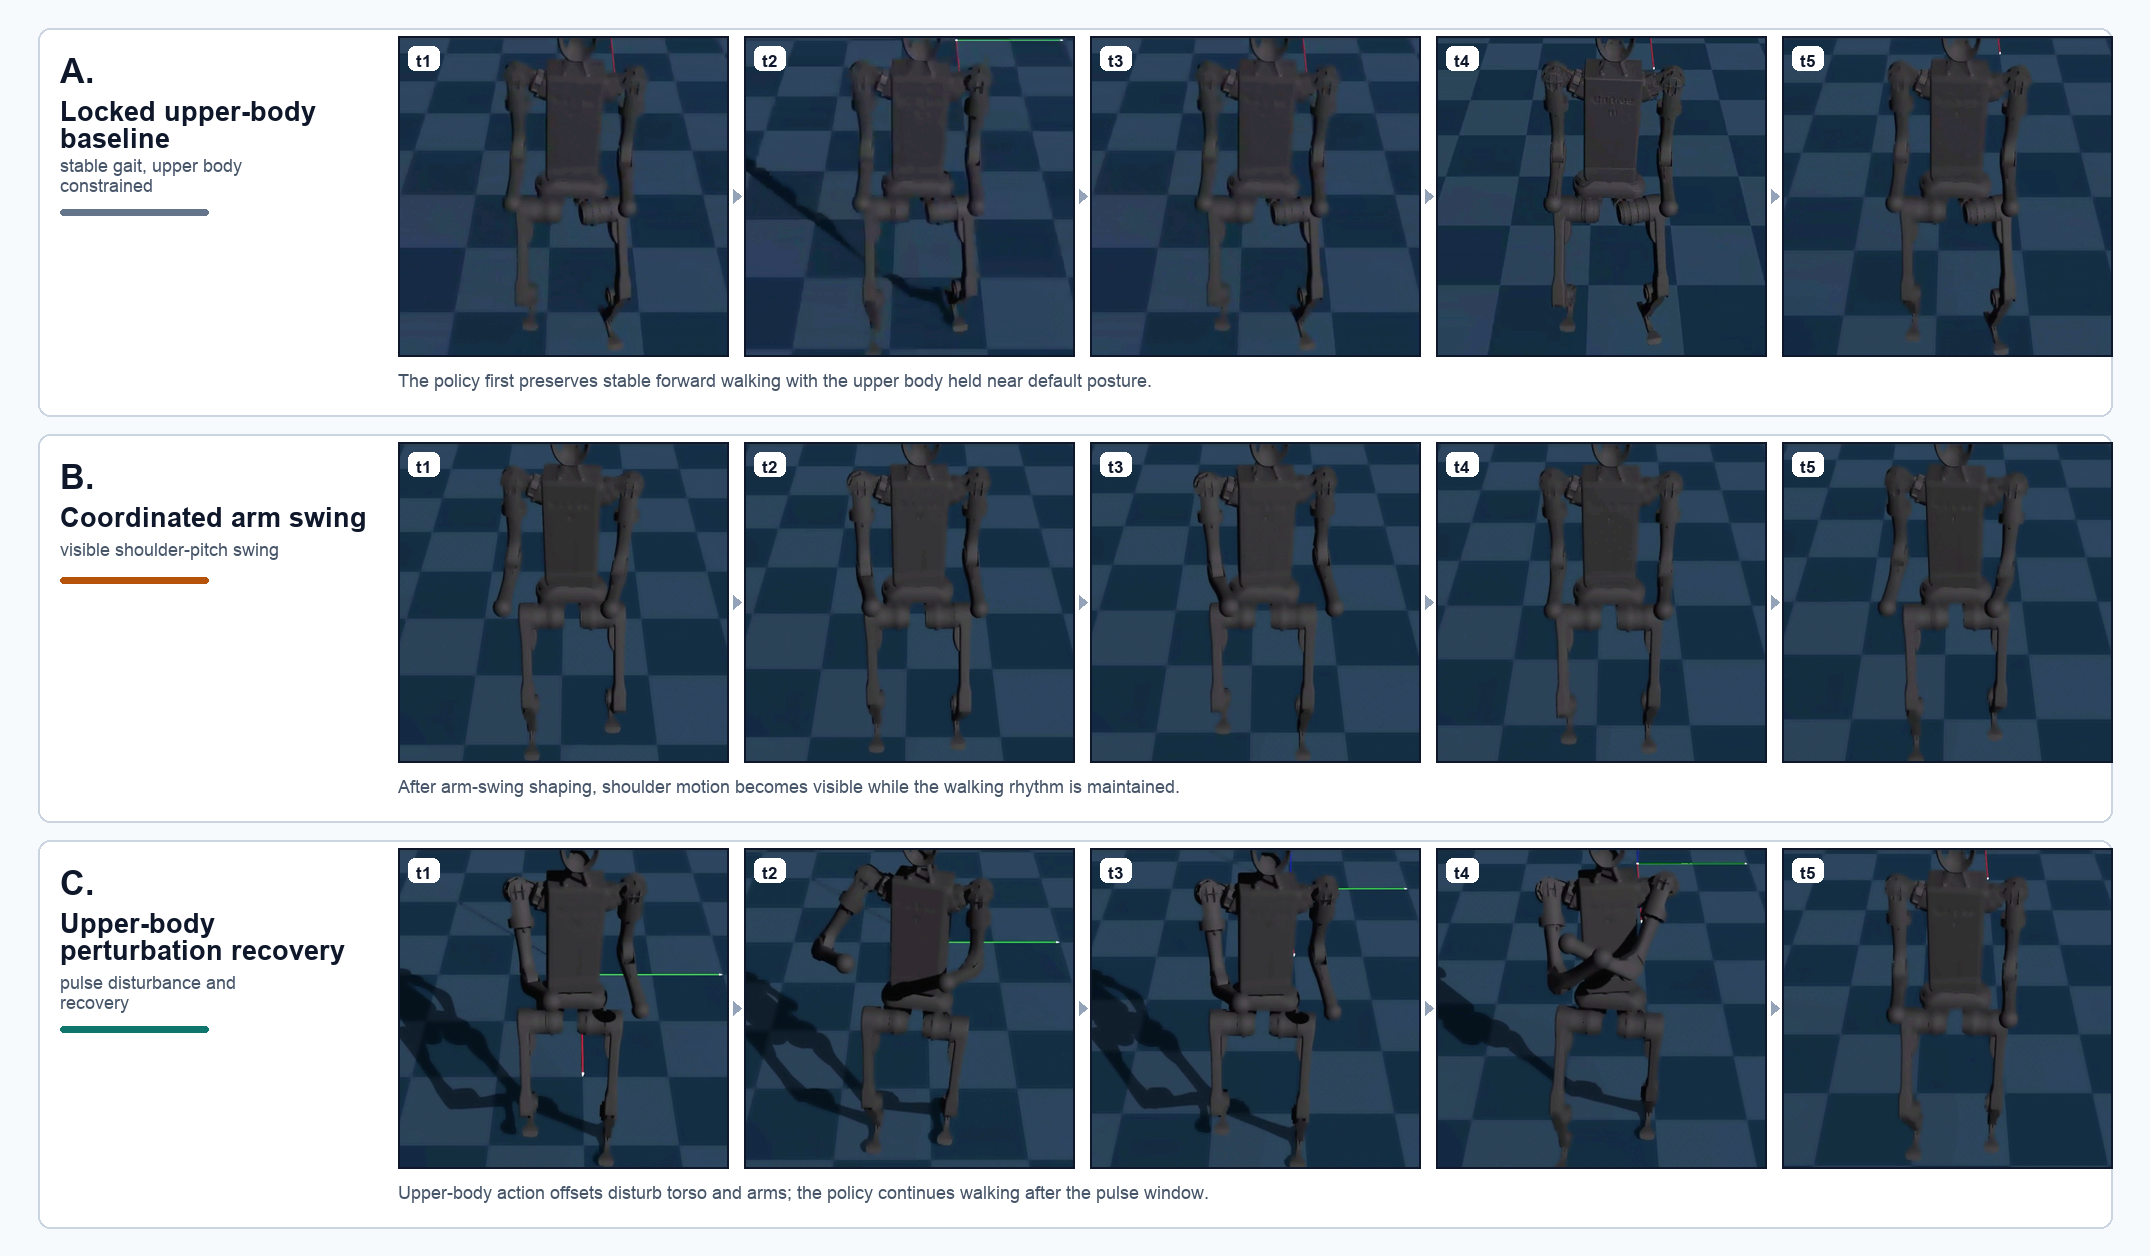
\includegraphics[width=\linewidth]{figure1_temporal_montage.png}
  \caption{三阶段行为证据。第一行展示上半身约束下的稳定行走；第二行展示直线行走中的可见肩部摆臂；第三行展示上肢脉冲扰动后的继续前进与恢复。}
  \label{fig:temporal}
\end{figure}

\section{问题建模}

本文将全身行走控制表述为部分可观测马尔可夫决策过程：
\begin{equation}
\mathcal{M}=(\mathcal{S},\mathcal{A},P,r,\gamma,p_0),
\end{equation}
其中 $s_t\in\mathcal{S}$ 表示机器人状态，$a_t\in\mathcal{A}$ 表示策略输出的关节动作，$P$ 为转移动力学，$r_t$ 为即时奖励，$\gamma$ 为折扣因子。策略 $\pi_\theta(a_t\mid o_t)$ 基于本体观测 $o_t$ 输出 19DoF 关节动作，优化目标为：
\begin{equation}
J(\theta)=
\mathbb{E}_{\pi_\theta}
\left[
\sum_{t=0}^{T-1}\gamma^t r_t
\right].
\end{equation}

动作空间可分为下肢集合 $\mathcal{L}$ 和上肢集合 $\mathcal{U}$：
\begin{equation}
\mathcal{A}=\mathcal{A}_{\mathcal{L}}\times\mathcal{A}_{\mathcal{U}},
\qquad
\mathcal{U}=\{\text{torso},\text{shoulder},\text{elbow}\}.
\end{equation}
训练目标不是最大化某个单一摆臂指标，而是在保持 locomotion 稳定的同时，使上肢动作满足步态协调和抗扰恢复约束。因此，奖励函数被设计为分阶段逐步扩展的组合目标。

\section{分阶段奖励设计}

\subsection{总体奖励分解}

本文采用如下统一奖励形式：
\begin{equation}
\begin{aligned}
r_t ={}&
r_t^{\mathrm{track}}
+ r_t^{\mathrm{safe}}
+ m_t^{\mathrm{stand}} r_t^{\mathrm{stand}}
+ m_t^{\mathrm{walk}} r_t^{\mathrm{walk}} \\
&+ m_t^{\mathrm{straight}} r_t^{\mathrm{swing}}
+ r_t^{\mathrm{robust}} .
\end{aligned}
\label{eq:reward-decompose}
\end{equation}
其中 $r_t^{\mathrm{track}}$ 表示速度和朝向跟踪，$r_t^{\mathrm{safe}}$ 表示姿态、关节限位、动作平滑和上肢安全约束；$r_t^{\mathrm{stand}}$、$r_t^{\mathrm{walk}}$ 和 $r_t^{\mathrm{swing}}$ 分别对应站立、行走和直线行走摆臂目标；$r_t^{\mathrm{robust}}$ 表示扰动阶段强化的稳定恢复目标。三个掩码 $m_t^{\mathrm{stand}}$、$m_t^{\mathrm{walk}}$、$m_t^{\mathrm{straight}}$ 使不同奖励项只在对应步态上下文中生效。

\begin{figure}[t]
  \centering
  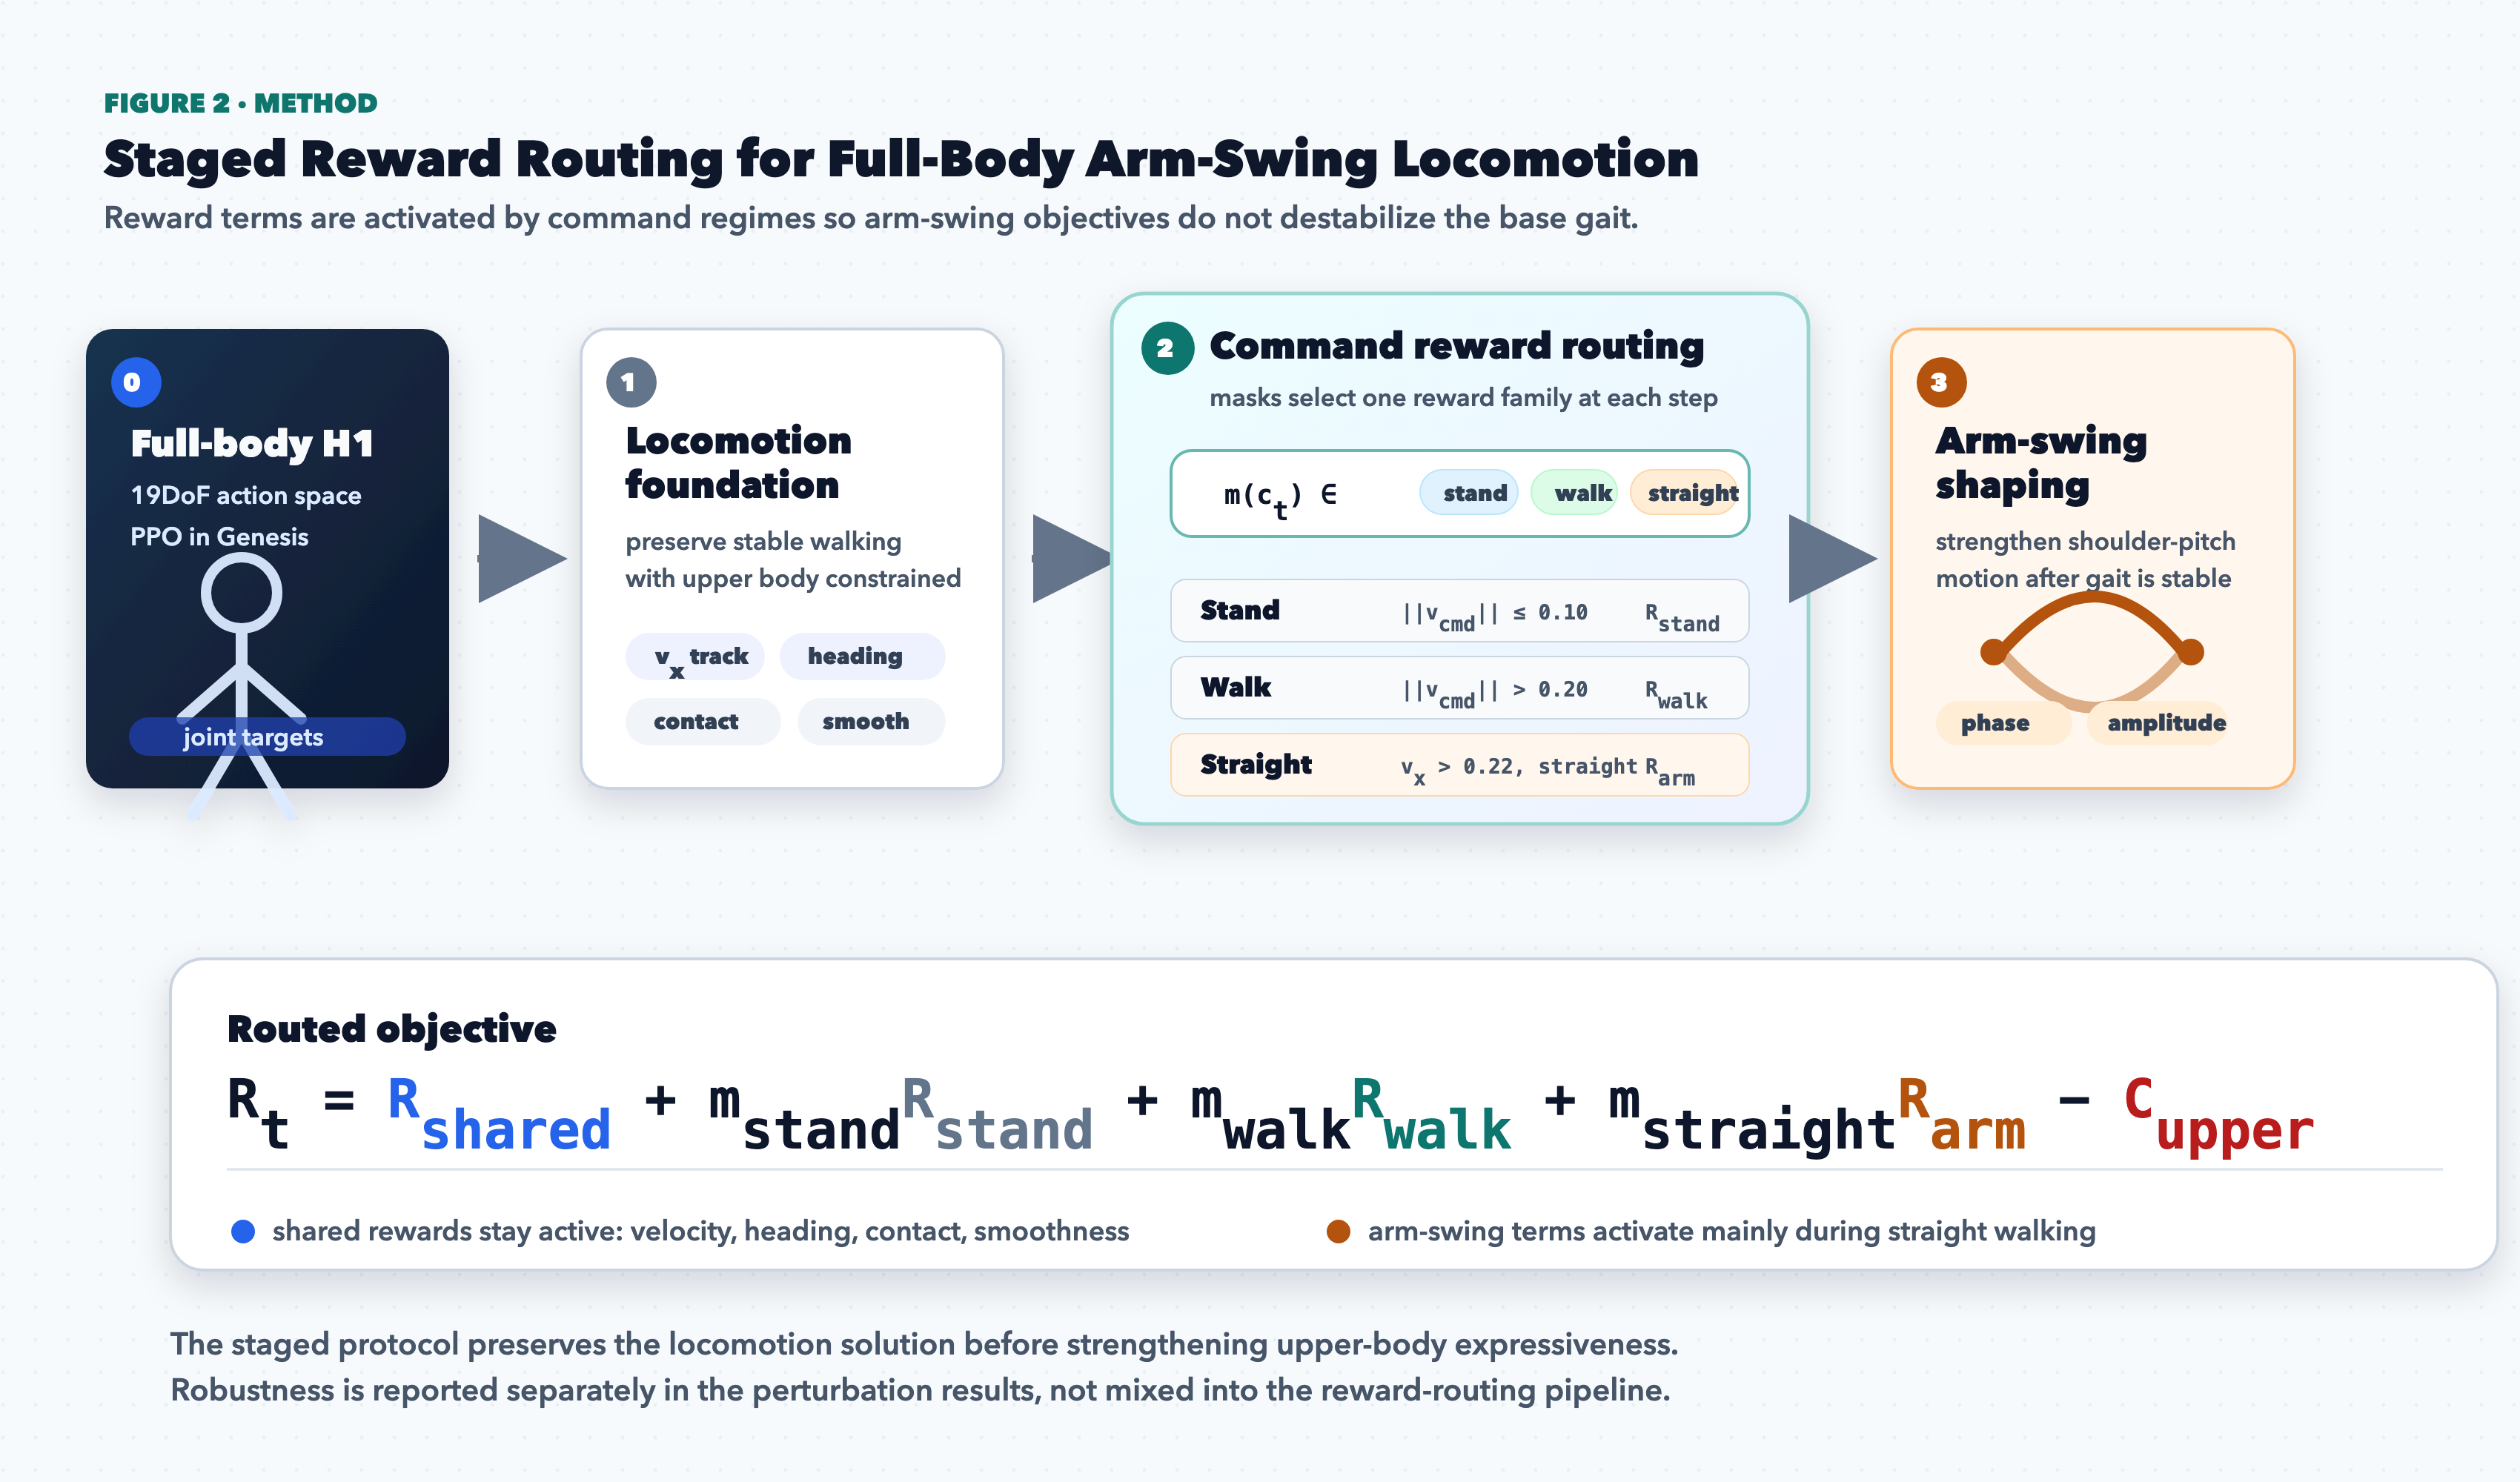
\includegraphics[width=0.95\linewidth]{staged_reward_routing.png}
  \caption{分阶段 reward routing 框架。策略首先在完整 19DoF 模型中保留稳定下肢 locomotion，随后通过命令条件化掩码激活步态相关奖励，最后在上肢动作通道加入脉冲扰动以评估和训练恢复能力。}
  \label{fig:routing}
\end{figure}

\subsection{Stage I：稳定下肢行走}

第一阶段的目标是在完整 19DoF 模型中建立稳定前向行走能力。尽管动作空间包含上肢关节，训练时仍将 torso、shoulder 和 elbow 约束在默认姿态附近。该阶段对应的奖励可概括为：
\begin{equation}
r_t^{(1)} =
r_t^{\mathrm{track}}
+ r_t^{\mathrm{base}}
+ r_t^{\mathrm{foot}}
- c_t^{\mathrm{upper-lock}}
- c_t^{\mathrm{smooth}} .
\end{equation}
其中速度与朝向跟踪项可写为：
\begin{equation}
r_t^{\mathrm{track}}
=
w_x \exp\left(-\frac{|v_{x,t}-v_{x,t}^{\mathrm{cmd}}|}{\sigma_x}\right)
+ w_\psi \exp\left(-\frac{|\psi_t-\psi_t^{\mathrm{cmd}}|}{\sigma_\psi}\right),
\end{equation}
而上肢锁定代价为：
\begin{equation}
c_t^{\mathrm{upper-lock}}
=
\sum_{j\in\mathcal{U}}
\relu{|q_{j,t}-q_j^0|-\epsilon_j}^2 .
\end{equation}
这里 $q_j^0$ 为默认关节角，$\relu{\cdot}=\max(\cdot,0)$。该设计使策略在全身模型中学习稳定 locomotion，但不允许上肢自由度参与早期探索，从而降低优化难度并避免上肢代偿。

\subsection{Stage II：命令条件化摆臂}

第二阶段在 Stage I 的基础上释放左右 shoulder pitch，并保持 torso、shoulder roll/yaw 和 elbow 的约束。该阶段的关键不是简单增大摆臂权重，而是将摆臂奖励路由到直线行走上下文中。命令条件化掩码定义为：
\begin{align}
m_t^{\mathrm{stand}}
&=
\ind\left[\left\|\mathbf{v}_{xy,t}^{\mathrm{cmd}}\right\|_2
\le v_{\mathrm{stand}}\right],\\
m_t^{\mathrm{walk}}
&=
\ind\left[\left\|\mathbf{v}_{xy,t}^{\mathrm{cmd}}\right\|_2
> v_{\mathrm{walk}}\right],\\
m_t^{\mathrm{straight}}
&=
\ind\left[
v_{x,t}^{\mathrm{cmd}}>v_{\min}
\land |v_{y,t}^{\mathrm{cmd}}|<\epsilon_y
\land |\omega_{z,t}^{\mathrm{cmd}}|<\epsilon_\omega
\right].
\end{align}

摆臂奖励由三个主要误差项构成。首先，肩部与对侧髋部的相位耦合为：
\begin{equation}
e_t^{\mathrm{phase}}
=
\left(q_{L,t}^{\mathrm{sh}}-k q_{R,t}^{\mathrm{hip}}\right)^2
+
\left(q_{R,t}^{\mathrm{sh}}-k q_{L,t}^{\mathrm{hip}}\right)^2 .
\end{equation}
其次，左右肩 pitch 速度应近似反相：
\begin{equation}
e_t^{\mathrm{opp}}
=
\left(\dot q_{L,t}^{\mathrm{sh}}+\dot q_{R,t}^{\mathrm{sh}}\right)^2 .
\end{equation}
最后，左右肘部末端在机器人基坐标系中的前后位移应达到最低可见摆幅：
\begin{equation}
e_t^{\mathrm{amp}}
=
\relu{
\delta_{\min}
-
\left|x_{L,t}^{\mathrm{elbow}}-x_{R,t}^{\mathrm{elbow}}\right|
}^2 .
\end{equation}
因此，第二阶段的摆臂项可写为：
\begin{equation}
r_t^{\mathrm{swing}}
=
-w_{\mathrm{phase}}e_t^{\mathrm{phase}}
-w_{\mathrm{opp}}e_t^{\mathrm{opp}}
-w_{\mathrm{amp}}e_t^{\mathrm{amp}},
\end{equation}
并通过 $m_t^{\mathrm{straight}}$ 只在直线前进命令下激活。这一设计借鉴了 gait-conditioned reinforcement learning 中的 reward routing 思想：不同状态下的行为目标不同，奖励也应随上下文切换。

\subsection{Stage III：上肢扰动恢复}

第三阶段继承第二阶段的摆臂目标，并在上肢动作通道加入随机脉冲扰动。设策略输出动作 $a_t$，执行动作 $\tilde a_t$ 定义为：
\begin{equation}
\tilde a_{t,j}=
\begin{cases}
\mathrm{clip}(a_{t,j}+s_j\eta_{t,j},-a_{\max},a_{\max}), & j\in\mathcal{U},\\
a_{t,j}, & j\in\mathcal{L},
\end{cases}
\end{equation}
其中 $\eta_{t,j}\sim\mathcal{U}(-\alpha,\alpha)$ 为随机动作偏移，$s_j$ 为不同上肢关节的扰动缩放系数，$\alpha$ 为扰动幅度。扰动采用 pulse 形式：在短时间窗口中保持随机偏移，然后关闭扰动并留出恢复窗口。该机制比连续噪声更适合考察恢复能力，因为它将“受扰”和“恢复”两个阶段显式分开。

第三阶段加强了直行和姿态稳定项：
\begin{equation}
r_t^{\mathrm{robust}}
=
w_v r_t^{v_x}
+ w_h r_t^{\mathrm{heading}}
-\lambda_o c_t^{\mathrm{orientation}}
-\lambda_y |v_{y,t}|
-\lambda_s \relu{v_{\min}-v_{x,t}} .
\end{equation}
该阶段并不追求更大摆臂，而是要求策略在上肢被随机 action offset 扰动后仍能保持前向速度、较小侧向漂移和受控姿态倾斜。

\section{与 gait-conditioned reward routing 的关系}

参考论文提出的核心观点是，多 gait 或多行为学习中的主要困难来自 reward interference：站立要求静止和双脚支撑，行走要求周期性足端摆动和前向速度，跑步要求更短接触和更强 push-off。若所有 gait-specific reward 同时生效，策略会收到互相矛盾的优化信号。该论文通过 gait ID 和 reward mask 实现动态 reward routing，使共享策略在不同 gait 下优化不同目标。

本文并未完整复现该论文的多 gait ID、LSTM 策略和 centroidal angular momentum reward，而是将其思想迁移为更轻量的 command-based routing。与原论文相比，本文任务只有站立、直线行走、摆臂和扰动恢复这几个上下文；因此可以直接由速度命令构造 mask，而不必扩展观测结构。该迁移保留了 reward routing 的关键优势：摆臂项不会在站立或复杂转向中强制激活，站立稳定项也不会在行走时压制必要的上肢协调。

\section{实验设置}

实验在 Genesis 仿真环境中训练 H1 19DoF 全身策略。评估使用 32 个并行环境，时间长度为 1000 step，即 20 s；命令速度为 $[0.6,0,0]$ m/s。扰动只施加于 torso、shoulder 和 elbow 动作通道，下肢动作不被直接扰动。本文报告三类指标。

存活率定义为：
\begin{equation}
S=\frac{1}{N}\sum_{i=1}^{N}\ind[T_i\ge T],
\end{equation}
其中 $T_i$ 为第 $i$ 个环境第一次非 timeout reset 的时间。前向速度误差定义为：
\begin{equation}
E_{v_x}=
\frac{1}{NT}
\sum_{i=1}^{N}\sum_{t=1}^{T}
\left|v_{x,t}^{(i)}-v_x^{\mathrm{cmd}}\right|.
\end{equation}
姿态倾斜由投影重力的水平分量近似：
\begin{equation}
\theta_t=
\arcsin\left(
\left\|\mathbf{g}_{xy,t}^{\mathrm{proj}}\right\|_2
\right).
\end{equation}
恢复成功率衡量每次扰动 pulse 结束后，机器人是否重新达到速度和姿态阈值：
\begin{equation}
\rho=
\frac{1}{K}
\sum_{k=1}^{K}
\ind
\left[
v_{x,t_k}^{\mathrm{rec}}\ge 0.8 v_x^{\mathrm{cmd}}
\land
\theta_{t_k}^{\mathrm{rec}}\le \theta_{\max}
\right].
\end{equation}

\section{结果}

\begin{figure}[t]
  \centering
  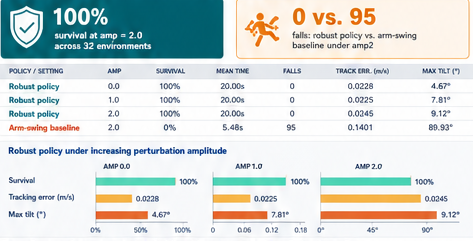
\includegraphics[width=0.95\linewidth]{poster3_element_22_quantitative_chart.png}
  \caption{有限时长扰动评估。最终鲁棒策略在扰动幅度增大到 2.0 时仍保持完整存活率和较低速度误差；未经过扰动鲁棒训练的摆臂策略在相同扰动下出现频繁跌倒。}
  \label{fig:quant}
\end{figure}

\begin{table}[t]
  \caption{上肢扰动下的有限时长评估结果。}
  \label{tab:robust}
  \centering
  \scriptsize
  \resizebox{\linewidth}{!}{%
  \begin{tabular}{lccccccc}
    \toprule
    策略 & 扰动幅度 $\alpha$ & 存活率 $\uparrow$ & 平均存活时间 $\uparrow$ & $E_{v_x}$ $\downarrow$ & 平均侧向速度 $\downarrow$ & 最大倾斜 $\downarrow$ & 总跌倒次数 $\downarrow$ \\
    \midrule
    Stage III & 0.0 & 100.0\% & 20.00 s & 0.0228 m/s & 0.0508 m/s & 4.67 deg & 0 \\
    Stage III & 1.0 & 100.0\% & 20.00 s & 0.0225 m/s & 0.0542 m/s & 7.81 deg & 0 \\
    Stage III & 2.0 & 100.0\% & 20.00 s & 0.0245 m/s & 0.0564 m/s & 9.12 deg & 0 \\
    Stage II baseline & 2.0 & 0.0\% & 5.48 s & 0.1401 m/s & 0.1335 m/s & 89.93 deg & 95 \\
    \bottomrule
  \end{tabular}}
\end{table}

\begin{table}[t]
  \caption{上肢摆臂相关指标。}
  \label{tab:armswing}
  \centering
  \scriptsize
  \resizebox{\linewidth}{!}{%
  \begin{tabular}{lccccc}
    \toprule
    策略 & 扰动幅度 $\alpha$ & 平均上肢动作扰动 & 肩部摆幅 & 左右臂反相误差 $\downarrow$ & 肘部末端前后位移 \\
    \midrule
    Stage III & 0.0 & 0.0000 & 0.2317 rad & 0.4239 rad & 0.1035 m \\
    Stage III & 1.0 & 0.1095 & 0.2141 rad & 0.3249 rad & 0.1098 m \\
    Stage III & 2.0 & 0.2168 & 0.2536 rad & 0.3952 rad & 0.1165 m \\
    Stage II baseline & 2.0 & 0.2079 & 0.2638 rad & 0.2997 rad & 0.1459 m \\
    \bottomrule
  \end{tabular}}
\end{table}

结果显示，Stage III 在扰动幅度 $\alpha=2.0$ 时仍保持 100\% 存活率，前向速度误差仅从无扰动时的 0.0228 m/s 增加到 0.0245 m/s，最大倾斜保持在 9.12 deg。相比之下，Stage II baseline 虽然已经具有可见摆臂，但在相同扰动下所有环境均发生失败，平均存活时间降至 5.48 s，并累计 95 次跌倒。表~\ref{tab:armswing} 进一步表明，Stage III 的鲁棒性并不是通过消除上肢运动获得的；在 $\alpha=2.0$ 时，策略仍保持 0.2536 rad 的肩部摆幅和 0.1165 m 的肘部末端前后位移。

\section{失败设计分析}

在最终三阶段方案形成之前，我们评估过多个探索性 reward 版本。这些版本没有稳定地产生自然摆臂，原因主要在于 reward 目标缺少上下文路由，或者摆臂信号与稳定性约束发生冲突。

\begin{table}[t]
  \caption{探索性失败阶段的主要问题。}
  \label{tab:failed}
  \centering
  \small
  \begin{tabularx}{\linewidth}{lXX}
    \toprule
    探索阶段 & 设计动机 & 主要问题 \\
    \midrule
    stage2 & 只释放 shoulder pitch，引入弱相位与末端约束 & 摆臂信号弱，容易被平滑、限位和回中项压制 \\
    stage3 & 进一步释放双臂，强化末端和横向限制 & 上肢 reward 过多且方向混杂，策略倾向僵硬或局部规避惩罚 \\
    stage4 & 使用固定正弦 teacher 直接塑造 shoulder pitch & teacher 与实际接触相位和速度命令不同步，易破坏步态自然性 \\
    stage5 & 降低 teacher 幅度，尝试更保守摆臂 & 摆臂信号进一步变弱，仍未解决全局 reward interference \\
    \bottomrule
  \end{tabularx}
\end{table}

这些失败表明，摆臂学习不能简化为“提高某个摆臂权重”。当站立、行走、转向和扰动恢复共享同一组全局 reward 时，策略会收到互相矛盾的梯度。有效设计需要首先保护 locomotion，再仅在直线行走时激活 arm-leg coordination，并在最后单独训练扰动恢复。

\section{讨论}

本文方法的优势在于其可解释性。每个阶段都对应明确的行为假设：Stage I 验证完整模型中的稳定下肢行走；Stage II 验证命令条件化 reward routing 能否产生可见摆臂；Stage III 验证该摆臂策略能否在上肢 action pulse 下恢复稳定。与使用 MoCap imitation 或 adversarial motion prior 的方法相比，本文不依赖外部动作数据，因此实现成本较低，且 reward 项与失败模式之间的关系更容易分析。

局限性也较明确。第一，本文仍然是手工 reward shaping，摆臂自然性由 shoulder pitch 相位、速度反相和末端位移近似描述，尚未显式优化全身 centroidal angular momentum。第二，实验仍局限于仿真短时评估，不能直接声称真实机器人迁移效果。第三，当前 routing 依赖速度命令阈值；如果任务扩展到复杂转向、变速或非平地行走，可能需要更丰富的 gait state 表示。

\section{结论}

本文提出了一种面向 H1 人形机器人的三阶段奖励课程，使策略从稳定下肢行走逐步过渡到自然摆臂，并进一步具备抵抗上肢随机动作扰动的能力。核心结论是：上肢摆臂应被视为步态条件化的全身协调行为，而不是孤立的关节轨迹跟踪问题。通过先约束上肢建立 locomotion 基础，再使用 command-based reward routing 激活直线行走摆臂目标，最后在动作层加入上肢 pulse 扰动训练恢复能力，最终策略在强扰动下仍保持完整存活率和低速度误差，同时保留可见摆臂。该结果支持了分阶段、上下文路由和鲁棒性评估相结合的 reward 设计路线。

\begin{thebibliography}{9}
\small

\bibitem{peng2025gait}
T. Peng, L. Bao, and C. Zhou.
\newblock Gait-conditioned reinforcement learning with multi-phase curriculum for humanoid locomotion.
\newblock 2025.

\bibitem{rudin2022learning}
N. Rudin, D. Hoeller, P. Reist, and M. Hutter.
\newblock Learning to walk in minutes using massively parallel deep reinforcement learning.
\newblock In \emph{Conference on Robot Learning}, 2022.

\bibitem{peng2019mcp}
X. B. Peng, M. Chang, G. Zhang, P. Abbeel, and S. Levine.
\newblock MCP: Learning composable hierarchical control with multiplicative compositional policies.
\newblock In \emph{NeurIPS}, 2019.

\bibitem{peng2021amp}
X. B. Peng, Z. Ma, P. Abbeel, S. Levine, and A. Kanazawa.
\newblock AMP: Adversarial motion priors for stylized physics-based character control.
\newblock \emph{ACM Transactions on Graphics}, 2021.

\bibitem{collins2009dynamic}
S. H. Collins, P. G. Adamczyk, and A. D. Kuo.
\newblock Dynamic arm swinging in human walking.
\newblock \emph{Proceedings of the Royal Society B}, 2009.

\end{thebibliography}

\end{document}
